% !Mode:: "TeX:UTF-8"
\subsection{Convergence Detection}

The graph is loopy in most scenarios, which might cause Belief Propagation could not converge. Although Yedidia had proposed a theory proving when Belief Propagation would converge and get acceptable results, it’s more practical to just run Belief Propagation and wait for it getting converged.

When running Belief Propagation, we can simply set the number of iterations after which BP terminates. And this is what PEGASUS’s implementation of BP currently using. The algorithm terminates after fixed number of iterations, without knowing whether it converged or not.

We found that it’s a bit difficult for us to tell whether we got the stable answer from BP when we evaluate BP on different datasets. The result would vary if we adjusted the number of iterations. So, we think convergence detection would be very helpful for users running BP on their datasets. It’s even essential for a BP implementation to produce the right answer.

Some discussions on convergence had been proposed by Mooij, they detect convergence by checking the difference between all the new messages and old messages. We followed their work and implemented convergence detection in the same way. Every iteration, we check the difference on every pair of new and old messages and the algorithm stops when all the differences are below threshold.

With above convergence detection mechanism, we can monitor the behavior of algorithm and tune the parameters and algorithm accordingly.

\subsection{Message Smoothing}

As discussed above, BP may not converge in some situations. If there are a lot of loops in the network, and even worse, many messages conflicts with their complement message from the other direction, there will be oscillatory behaviors during the message updating process and make BP never converge. To tackle this problem, Pretti found a method named message smoothing. We implemented this algorithm on BP.

It reduces oscillatory behaviors in the message updating process by smoothing, or damping, messages between two iterations. In the original belief propagation, the messages which node $i$ will send to other nodes are a function of messages sent to node $i$, which may cause oscillations in loopy networks. We can avoid changing messages too drastically by having a weighted average of the new message and the old message as follows. This can dampen oscillations and increase the chances that it converges.

Denoting $\bar{m}_{i,j}^{t}(x_{j})$ as the updated message in iteration t obtained by message passing, $\lambda$ as the message smoothing factor, the new message from node $i$ to node $j$ in iteration $t$, denoted by $m_{i,j}^{t}(x_{j})$ is computed as weighted average of the old message and the updated message as
\begin{equation}
    m_{i,j}^{t}(x_{j}) = (1-\lambda)m_{i,j}^{t-1}(x_{j}) + \lambda\bar{m}_{i,j}^{t}(x_{j})
\end{equation}

\subsection{Methods for Extending Fast BP to Multiclass Problems}

\subsubsection{Error Correcting Code Methods}

\subsubsection*{Motivation}
Fast BP is now limited to solve problems with only 2 labels. Formally extending Fast BP to multiclass can be difficult. Instead of formally formulating the multiclass Fast BP, we emphasize BP as a tool to give the correct label rather than compute the probability. Thus we can divide a single multiclass problem into several binary problems so that we can use Fast BP to give the label.


\subsubsection*{General Definition}

To solve a multiclass problem, which has $k$ classes and $l$ training example $(x_{1},y_{1})...(x_{l},y_{l})$, we can use error correcting code approach, which usually involves the following steps:

\subsubsection*{Code Design}

In this step, for each class in the $k$ classes, we design a unique $N$ bits code. For example, for a problem recognizing hand writings of 10 digits, we can define the following 6 bits error codes, shown in Figure 1.

\begin{figure}[!htbp]
\centering
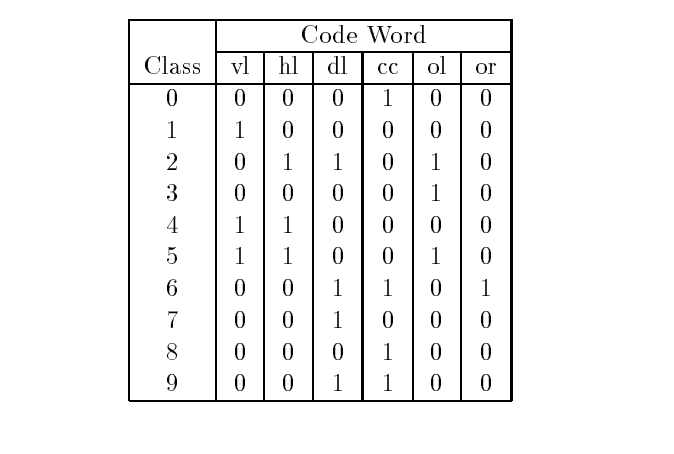
\includegraphics[bb=0 0 680 500,scale=.3]{FIG/code.png}
\caption{Coding scheme for 10 digits recognizing problem}
\end{figure}

The meaning of those codes follows the description in the figure 2 from \cite{Thomas1995}.


\begin{figure}[!htbp]
\centering
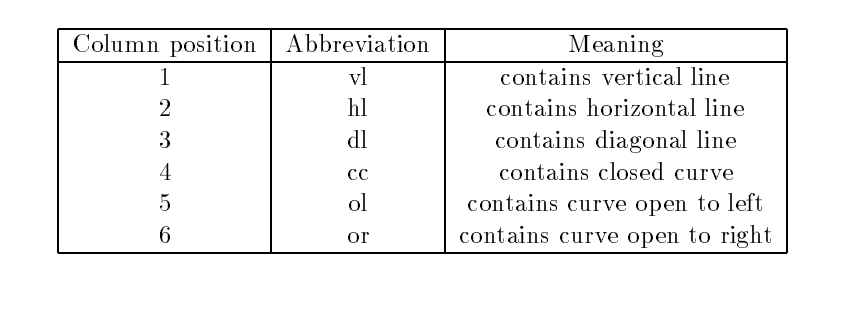
\includegraphics[bb=0 0 860 300,scale=.3]{FIG/meaning.png}
\caption{Meaning of each bit}
\end{figure}

There are basically two principles for design a code\cite{Thomas1995}:
\begin{enumerate}
    \item \textbf{Row Distance}: The hamming distance between each two classes' codes should be as large as possible to make classes more distinguishable from each other.
    \item \textbf{Column Distance}: Each bit classifier should be independent from each other.
\end{enumerate}

It is obvious that there is a trade-off between those two principles, which leads to different code design methods. We will adapt the one described in Thomas's Paper\cite{Thomas1995}, which is every effective to generate compact yet distinguish code.

\subsubsection*{Running Fast BP for Bits}

As we already described in the previous sections, after designing of code, we run Fast BP for each bits, note as $f_{1}...f_{n}$. We can interpret $f_{i}(x)$ as the probability that the number appear on the $i^{th}$ bit of the code for a given example $x$ is 1.

\subsubsection*{Deciding Label}

For a node $r$, after computation, we get a vector of predictions of those functions:

\begin{gather*}
    f(r) = (f_{1}(r)...f_{n}(r))
\end{gather*}


In order to make final prediction we should find the class which is \textit{closest} to $f(r)$.

In general, there are different approaches to achieve this:

\begin{enumerate}
    \item \textbf{Hamming Decoding}: Transform $f(r)$ from real-value to binary value, and calculate the Hamming distance with code of each class. The label that has the shortest hamming distance is chosen.
    \item \textbf{Loss-based Decoding}: This method is introduced in \cite{Erin2000}, which defines a loss function between probability made by $f$ and the target bit of class, without transform $f(r)$ into binaries.
\end{enumerate}

\subsubsection*{Practical Variations of ECOC}

Error correcting code suffers from one major disadvantage, that is, if the number of classes is large, the number of bits will grow excessively, even exponentially. Sometimes, if the classification algorithm itself is time-consuming, such as Fast BP, even the number of bits is reasonable, ECOC becomes very expensive.

So we introduce a practical variation of ECOC, called One-VS-All schema. In \cite{Erin2000}, One-VS-All is proved to be a special case of ECOC.

It follows a very simple strategy: for every class, we train a binary classifier to distinguish whether a node is a class or not. The decision of final label is simple too, we just pick the class that has the highest $YES$ probability. One-VS-All will significantly reduce the number of bits involved, especially when $k$ is large. And as \cite{Ryan2000} suggests, when the underlying binary classifier performs well, One-VS-All works as well as ECOC approach.

%\begin{enumerate}
%   \item \textbf{One-Vs-All}: In this scheme every class is associated with a classifier that tells whether an incoming example is in this class or not. The final prediction is made according to some predefined decision value, like probability given by Logistics Regression.
%   \item \textbf{All-Vs-All}: A classifier is trained for every pair of classes. As there are $O(n^{2})$ classifiers to train, some algorithms are introduced to reduce the number of classifier pairs\cite{Platt2000}
%\end{enumerate}

Actually, the two schemes are just special case of ECOC, but are much more straight forward.


\subsection{FastBP for Multiple Classes}
The original Belief propagation update rules are as follows:

\begin{equation}
\label{eq:origbp_b}
b_i(x_k) = \eta\cdot \phi_i(x_k)\cdot\mathop{\prod}_{j\in N(i)}m_{ij}(x_k)
\end{equation}
\begin{equation}
\label{eq:origbp_m}
m_{ij}(x_g)=\mathop{\sum}_{x_k}\phi_{i}(x_g)\cdot \psi_{ij}(x_k,x_g)\cdot\mathop{\prod}_{n\in N(i)\setminus j} m_{ni}(x_k)
\end{equation}

where $x_k$ is one state for any node and $b_i(x_k)$ is the probability (belief) for node $i$ staying at state $x_k$. So the first step of approximating the original rules is to remove the product operators. A very intuitive and common method is taking logarithms of both sides. For Eq.(\ref{eq:origbp_b}), it becomes
\begin{equation}
\log(b_i(x_k)) = \log(\eta) + \log(\phi_i(x_k)) + \mathop{\sum}_{j\in N(i)}\log(m_{ij}(x_k))
\end{equation}

Like the work~\cite{KoutraKKCPF11} by Koutra, et al., we have to use a smart approximation for the logarithm. But let us skip this part for a moment. Assume we have a reasonable approximation of logarithms now, i.e. $F(v)\approx \log(v)$, if $v$ is a vector, then $F(v)$ is also a vector whose each component is the approximation of the logarithm of corresponding $v$'s component.

So we can rewrite Eq.(\ref{eq:origbp_b}) as $F(b_i(x_k))=C_{ik}+\mathop{\sum}_{j\in N(i)}F(m_{ij}(x_k))$, where $C_{ik}=\log\eta + \log(\phi_i(x_k))$. Moreover, we use $\mathbf{b_i}$ as the status vector of beliefs of node $i$. For simplicity, assume there are only three classes, $x_k\in \{x_1, x_2, x_3\}$, i.e. $\mathbf{b_i} = \left[ \begin{array}{c}
b_i(x_1) \\
b_i(x_2) \\
b_i(x_3) \end{array} \right]$ we can get the general equation for any node $i$,

\begin{equation}
F(\mathbf{b_i})=
\left( \begin{array}{cccc}
F(\mathbf{m_{i1}})&F(\mathbf{m_{i2}})&\cdots& F(\mathbf{m_{in}})\end{array} \right)\mathbf{A_i}+\mathbf{C_i}
\end{equation}

where $\mathbf{A_i}$ is the $i$th column of the adjacency matrix and $\mathbf{C_i} = \left[ \begin{array}{c}
C_{i1} \\
C_{i2} \\
C_{i3} \end{array} \right]$
and $\mathbf{m_{ij}} = \left[ \begin{array}{c}
m_{ij}(x_1) \\
m_{ij}(x_2) \\
m_{ij}(x_3) \end{array} \right]$, Now, replace $\phi_i(x_k)\prod_{n\in N(i)\setminus j} m_{ni}(x_k)$ with $b_i(x_k)/(\eta m_{ji}(x_k))$, Eq.(\ref{eq:origbp_m}) can be rewritten as $m_{ij}(x_k) = \sum_{x_g}\psi_{ij}(x_k,x_g)b_i(x_k)/(\eta m_{ji}(x_k))$, which means
\begin{equation}
\mathbf{m_{ij}} = \frac{1}{\eta} \Psi_{ij} \left[ \begin{array}{c}
b_i(x_1)/m_{ji}(x_1) \\
b_i(x_2)/m_{ji}(x_2) \\
b_i(x_3)/m_{ji}(x_3) \end{array} \right]
\end{equation}


where $\Psi$ is the correlation (transition) matrix of every two nodes, i.e., under the three class assumption,
\begin{equation}
\Psi_{ij} = \left[ \begin{array}{ccc}
\psi_{ij}(x_1,x_1)&\psi_{ij}(x_1,x_2)&\psi_{ij}(x_1,x_3) \\
\psi_{ij}(x_2,x_1)&\psi_{ij}(x_2,x_2)&\psi_{ij}(x_2,x_3) \\
\psi_{ij}(x_3,x_1)&\psi_{ij}(x_3,x_2)&\psi_{ij}(x_3,x_3) \end{array} \right]
\end{equation}

It can also be written as
\begin{equation}
\mathbf{m_{ij}} = \frac{1}{\eta} \Psi_{ij} \left[ \begin{array}{ccc}
1/m_{ji}(x_1)&0&0 \\
0 &1/m_{ji}(x_2)&0 \\
0& 0 &1/m_{ji}(x_3) \end{array} \right] \left[ \begin{array}{c}
b_i(x_1)\\
b_i(x_2)\\
b_i(x_3)\end{array} \right]
\end{equation}

Suppose all nodes are homogeneous, i.e. $\forall i,j$ , $\Psi_{ij} = \Psi$ is non-singular (which is also the common case), then we get a relation between the state of one node and two different direction messages on its one edge (since $\eta$ is just a normalization constant, we ignore $\eta$ in the following analysis):
\begin{equation}
\mathbf{b_i} = diag(\mathbf{m_{ji}})\Psi^{-1}\mathbf{m_{ij}}
\end{equation}

Finally, we get the matrix equations for belief propagation,
\begin{equation}
\label{equ:bfnewrule_b}
\mathbf{b_i} = diag(\mathbf{m_{ji}})\Psi^{-1}\mathbf{m_{ij}}~~~~\forall i\in [n],~j\in N(i)
\end{equation}

\begin{equation}
\label{equ:bfnewrule_m}
F(\mathbf{b_i})=
\left( \begin{array}{cccc}
F(\mathbf{m_{i1}})&F(\mathbf{m_{i2}})&\cdots& F(\mathbf{m_{in}})\end{array} \right)\mathbf{A_i}+\mathbf{C_i}~~~\forall i\in [n]
\end{equation}

\subsubsection{Simple correlation matrix case}

In many cases, one node is inclined to connect with other nodes which are in the same class as itself. For example, when we buy a book in Amazon, it is very possible that we also buy another book, which has close relation with the first one (e.g. supplementary textbook), or the one that is suggested by the suggestion system. Another instance is that when we post a scenery photo on facebook, it is very likely that at the same time you will post more scenery photos instead of other kinds of photos. Based on this fact, we assume a simple case that the correlation matrix is almost as an identity matrix. In this case, $\Psi^{-1} \approx \mathbf{I}$, then

\begin{equation}
\label{equ:simplecorrelation}
\mathbf{b_i} \approx diag(\mathbf{m_{ji}})\mathbf{m_{ij}} = \mathbf{m_{ji}}\circ \mathbf{m_{ij}}
\end{equation}

where ``$\circ$'' is the hadamard product (element-wise product). However, the identity correlation matrix has a problem: if the graph is a strong connected graph, there is no feasible solution exists according to Eq.(\ref{equ:simplecorrelation}), since all the nodes are connected and they can only all belong to the same class. To avoid this problem, we allow the deviation for all beliefs,
$$\mathbf{b_i}  \leq \mathbf{m_{ji}}\circ \mathbf{m_{ij}} + \mathbf{s_i}$$
and $\mathbf{s_i} \geq 0$, i.e. every entry of $\mathbf{s_i}$ is greater than $0$. But put penalty on these slack variables. Also note that $\mathbf{m_{ij}}$ and $\mathbf{m_{ji}}$ always come in pairs, we can use $\mathbf{m'_{ij}} ~(= \mathbf{m'_{ji}})$ to replace $\mathbf{m_{ji}}\circ \mathbf{m_{ij}} ~(= \mathbf{m_{ij}}\circ \mathbf{m_{ji}})$, so basically we need to solve this optimization problem,
\begin{equation}
\begin{aligned}
& \underset{\mathbf{s}}{\text{minimize}}
& & \frac{1}{2}\mathop{\sum}_{k \in [n]\setminus V_0, j\in N(k)}||\mathbf{b_k} - \mathbf{m'_{kj}}||^2 + \frac{\lambda}{2}\sum_i||\mathbf{s_i}||^2 \\
& \text{subject to}
& &  \mathbf{b_i}-\mathbf{s_i} \leq \mathbf{m'_{ij}}, ~~\; i \in V_0, j\in N(i)\\
& &  &\mathbf{s_i}\geq 0 ~~\; i \in V_0\\
& &  &\mathbf{b_i}\geq 0 ~~\; i \in [n]\setminus V_0\\
& &  &\mathbf{m'_{ij}}\geq 0 ~~\; i \in [n], j\in N(i)
\end{aligned}
\end{equation}
Note that the node set $V_0$ is the labeled node set, i.e. $\mathbf{b_i}$, $i\in V_0$ is given. $\lambda$ is the adjustable weight which determines the importance of the deviation in our final result. If we want more initial labeled nodes can fit in this model, then give a larger value to $\lambda$, but meanwhile the estimation of the target nodes' beliefs tend to become worse.

Add lagrangian multiplier $\alpha_{ij} \geq 0$, $\beta_i \geq 0$, $\mu_i \geq 0$ and $\nu_i\geq 0$, $i\in V_0$, $j\in N(i)$  here, we get

\begin{align*}
&\frac{1}{2}\mathop{\sum}_{k \in [n]\setminus V_0, j\in N(k)}||\mathbf{b_k} - \mathbf{m'_{kj}}||^2 + \frac{\lambda}{2}\sum_i||\mathbf{s_i}||^2 + \mathop{\sum}_{i\in V_0,j\in N(i)}\alpha_{ij}(\mathbf{b_i}
-\mathbf{s_i} -  \mathbf{m'_{ij}}) \\&- \sum_i \beta_{i}\mathbf{s_i} - \sum_{i\in [n]\setminus V_0} \mu_{i}\mathbf{b_i} - \sum_{i\in [n], j\in N(i)} \nu_{i}\mathbf{m'_{ij}}
\end{align*}



It is easy to see that this optimization problem is a convex optimization problem, but we also need to assume there are positive feasible solution (i.e. strong convexity of optimization problem). Then according to the Karush-Kuhn-Tucker (\textbf{KKT}) conditions, we can get the global optimal solution.
\begin{align}
\label{equ:kkt1}
&\mathbf{b_k} - \mathbf{m'_{kj}} - \mu_k\vec{1} = 0 ~~~~&\forall k\in [n]\setminus V_0, j\in N(k)\\
\label{equ:kkt2}
&- \mathbf{b_k} + \mathbf{m'_{kj}} - \alpha_{jk}\vec{1} - \nu_{k}\vec{1} = 0 &\forall k\in [n]\setminus V_0, j\in N(k)~~and~~j\in V_0\\
\label{equ:kkt3}
&- \mathbf{b_k} - \mathbf{b_j} + 2\mathbf{m'_{kj}} - \nu_{k}\vec{1} = 0 &\forall k\in [n]\setminus V_0, j\in N(k)~~and~~j\in [n]\setminus V_0\\
\label{equ:kkt4}
& \alpha_{ij} = \alpha_{ji} = 0 &\forall i\in V_0, j\in N(i)~~and~~j\in V_0\\
\label{equ:kkt5}
&\lambda \mathbf{s_i} - \sum_{j\in N(i)}\alpha_{ij}\vec{1} - \beta_i \vec{1}=0 &\forall i\in V_0\\
\label{equ:kkt6}
&\alpha_{ij}(\mathbf{b_i}-\mathbf{s_i}- \mathbf{m'_{ij}}) = 0 &\forall i\in V_0, j\in N(i)\\
\label{equ:kkt7}
&\beta_i \mathbf{s_i} = 0 &\forall i\in V_0\\
\label{equ:kkt8}
&\mu_i \mathbf{b_i} = 0 &\forall i\in [n]\setminus V_0\\
\label{equ:kkt9}
&\nu_i \mathbf{m'_{ij}} = 0 &\forall i\in V_0, j\in N(i)
\end{align}

Even though it seems very complicated, all of these equations are very simple, and we need all of these equations to get the optimal result.  Eq.(\ref{equ:kkt1})$\sim$ Eq.(\ref{equ:kkt4}) are from the stationary condition of \textbf{KKT} condition, which describe the relationship between any two nodes (there are three kinds of node pair $(i,j)$ (1) $i,j$ are both labeled nodes in $V_0$, ; (2) one of $i,j$ is labeled node and another one is the target node; (3) $i,j$ are both target nodes. The belief results are all $\mathbf{b_k}$, $k\in [n]\setminus V_0$.

\subsubsection{Extended correlation matrix case}

Before we talk about the common correlation matrix, we should think about why the optimization problem proposed above works. See Fig.~\ref{fig:bpexample} for an example part of a small \textbf{BP} network. The idea of the previous optimization problem comes from ignoring the real value of the $m_{ij}$ and $m_{ji}$, but using a generalized variable $m'_{ij}$ to describe the relationship between two nodes $i$ and $j$.

Assume node $i$ is a labeled node, i.e. $\mathbf{b_i}$ is known, according to last subsection, the value of $\mathbf{m'_{ij}}$ can be bounded by $\mathbf{b_i}$ and $\mathbf{s_i}$. On the other hand, if node $j$ is an unknown (target) node, $\mathbf{b_j}$ can also be bounded by $\mathbf{m'_{ji}}$ and $\mathbf{s_j}$. The key point here is that $\mathbf{m'_{ij}} = \mathbf{m'_{ji}}$. This equation means we can approximate $\mathbf{b_j}$ with $\mathbf{b_i}$, $\mathbf{s_i}$ and $\mathbf{s_j}$. $\mathbf{s_i}$ and $\mathbf{s_j}$ are just the slack variables we defined, and we minimize all the slack variables in the objective functions. In one word, the captured relation between $\mathbf{m'_{ij}}$ and $\mathbf{m'_{ji}}$ can be used to describe the relation between $\mathbf{b_i}$ and $\mathbf{b_{j}}$, which is the objective to be optimized.

\begin{figure}[!htb]
\begin{center}
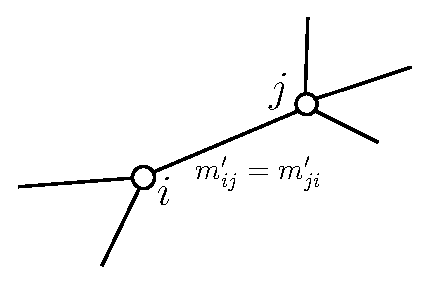
\includegraphics[scale=0.8]{FIG/bpexample}
{\caption{Small example of BP network}\label{fig:bpexample}}
\end{center}
\end{figure}

Recall that we actually use $\mathbf{m'_{ij}}$ to replace $diag(\mathbf{m_{ji}})\Psi^{-1} \mathbf{m_{ij}}$. Obviously that $\mathbf{m'_{ij}} = \mathbf{m'_{ij}}$ does not hold for common correlation matrix $\Psi$. But if we have

$$\mathbf{m'_{ij}} \approx \mathbf{m'_{ji}}$$
which holds in some cases, for instance that if $\Psi$ is close to $\mathbf{I}$. This assumption means that the analysis in the simple correlation matrix case still works. Also, we need to think about that why the slack variables $\mathbf{s_i}$, $i\in [n]/V_0$ are necessary. Simply speaking, the main reason is that we just use Eq.(\ref{equ:bfnewrule_b}) without Eq.(\ref{equ:bfnewrule_m}) to formulate the optimization problem. Although Eq.(\ref{equ:bfnewrule_b}) is derived by substituting $\phi_i(x_k)\prod_{n\in N(i)\setminus j} m_{ni}(x_k)$ with $b_i(x_k)/(\eta m_{ji}(x_k))$, which comes directly from Eq.(\ref{equ:bfnewrule_m}), we still lose parts of all the information of the original belief updating rule.

Due to the limitation of time, there are still two unsolved problems which can be interesting topics for further study. The first one is that we provide an equation system which is used to solve the optimization problem. How to organize these equations into a more concise form is not a easy task. The second problem, how can we derive an upper bound for the distance between the solution to the optimization problem and the solution of the original Belief Propagation algorithm. For example, if we are given $||\mathbf{m'_{ij}} - \mathbf{m'_{ji}}||_F^2 \leq \epsilon$, (here is the componentwise norm, i.e. Frobenius norm), we hope to derive an error upper bound as a function of $\epsilon$. Since we do not have time to implement some experiments to test the accuracy of this method, testing this result on different networks may be the next step.

\subsubsection{Quadratic approximation}
We also try another direction (relaxing the approximation assumption) to extend the \textbf{FaBP}, even though we do not really figure it out. A significant fact of the original \textbf{FaBP} algorithm is the assumption that all parameters are ``about half'', i.e. close to 1/2. This assumption provides a foundation for the correctness of Maclaurin series expansion used in the analysis. However, when there are more than two classes, without the concept of odd-ratio, we cannot achieve the similar assumption for any parameter. But we can use the quadratic approximation, i.e. second order Taylor approximation for the logarithms, i.e. instead of using $\log(x) \approx \log(1)+\log^{\prime}(1)(x-1)$ with the assumption that $x$ (the odd-ratio) is close to $\frac{1}{2}$, we use
$$\log(x)\approx \log(1)+\log^{\prime}(1)(x-1)+\frac{\log^{\prime\prime}(1)}{2}(x-1)^2$$
without the ``about half'' assumption.

More precisely, in Eq.(\ref{equ:bfnewrule_m}), $F(v) = (v - 1) - \frac{(v -1)^2 }{2}$

Still, for simplicity we assume there are three states for the node, i.e. $x_k\in \{x_1, x_2, x_3\}$. Then the left hand side of Eq.~(\ref{equ:bfnewrule_m}) is
\begin{equation}
\left[ \begin{array}{c}
b_i(x_1) \\
b_i(x_2) \\
b_i(x_3) \end{array} \right]
\circ
\left[ \begin{array}{c}
2-\frac{1}{2}b_i(x_1) \\
2-\frac{1}{2}b_i(x_2)\\
2-\frac{1}{2}b_i(x_3)\end{array} \right]
-
\left[ \begin{array}{c}
\frac{1}{2} \\
\frac{1}{2} \\
\frac{1}{2} \end{array} \right]
=
diag(\mathbf{b_i})(
\left[ \begin{array}{c}
2\\
2\\
2\end{array} \right]
-\frac{1}{2}\mathbf{b_i})
-
\left[ \begin{array}{c}
-\frac{1}{2} \\
-\frac{1}{2} \\
-\frac{1}{2} \end{array} \right]
\end{equation}

note that
\begin{equation}
diag(\mathbf{b_i}) \vec{\mathbf{1}}= \left[ \begin{array}{ccc}
b_i(x_1)&0&0 \\
0&b_i(x_2)&0 \\
0&0&b_i(x_3) \end{array} \right]\vec{\mathbf{1}}= \mathbf{b_i}
\end{equation}

Finally we get
\begin{equation}
\label{eq:newquadraticapprox}
diag(\mathbf{b_i})
(2\cdot\vec{\mathbf{1}}
-\frac{1}{2}\mathbf{b_i})-
\frac{1}{2}\vec{\mathbf{1}}
= \left( \begin{array}{cccc}
\mathbf{M_{i1}}&\mathbf{M_{i2}}&\cdots& \mathbf{M_{in}}\end{array} \right)\mathbf{A_i}+\mathbf{C_i}
\end{equation}

where $\mathbf{M_{ij}}$ can also be written as
$diag(\mathbf{m_{ij}})(2\cdot \vec{\mathbf{1}}-\frac{1}{2}\mathbf{m_{ij}})-\frac{1}{2}\vec{\mathbf{1}}$.

This new equation is still very complicated. But since the ``about-half'' assumption has been removed from this updating rule, it also has potential to be used in formulating a optimization problem as we discussed in previous sections, and if it can be done, the accuracy of the optimization problem will be definitely improved. Even though we cannot find a good usage for this new approximation of the belief updating rule now, we still believe it is an attemptable research point.

